\documentclass{article}%
\usepackage[T1]{fontenc}%
\usepackage[utf8]{inputenc}%
\usepackage{lmodern}%
\usepackage{textcomp}%
\usepackage{lastpage}%
\usepackage[head=40pt,margin=0.5in,bottom=0.6in]{geometry}%
\usepackage{graphicx}%
%
\title{\textbf{Denuncian intento de invasión en terreno de Terrazas de Bella Vista}}%
\author{MIGDALIS CAÑIZALEZ V.}%
\date{02/12/2018}%
%
\begin{document}%
\normalsize%
\maketitle%
\textbf{URL: }%
http://www.eluniversal.com/caracas/27245/denuncian{-}intento{-}de{-}invasion{-}en{-}terreno{-}de{-}terrazas{-}de{-}bella{-}vista\newline%
%
\textbf{Periodico: }%
EU, %
ID: %
27245, %
Seccion: %
caracas\newline%
%
\textbf{Palabras Claves: }%
NO\_TIENE\newline%
%
\textbf{Derecho: }%
2.8, %
Otros Derechos: %
, %
Sub Derechos: %
2.8.1.2\newline%
%
\textbf{EP: }%
NO\newline%
\newline%
%
\textbf{\textit{Los vecinos temen que ante la proximidad de las elecciones municipales se incrementen las invasiones en muchas zonas de Caracas  promovidas por los mismos candidatos.}}%
\newline%
\newline%
%
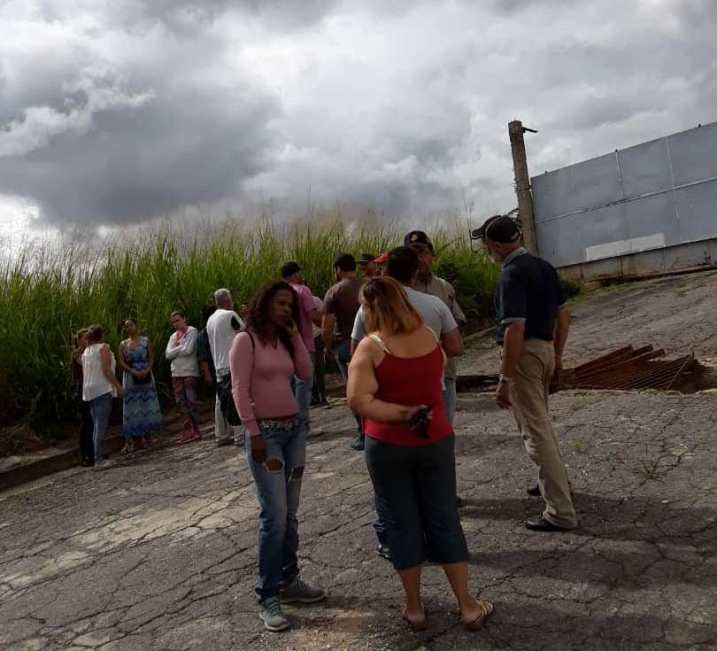
\includegraphics[width=300px]{260.jpg}%
\newline%
%
Vecinos de esta zona del oeste de Caracas denunciaron que ayer en horas de la mañana unas personas a bordo de tres camionetas, supuestamente haciéndose pasar por funcionarios de la alcaldía de Caracas ingresaron a la urbanización~ para invadir unos terrenos en la zona protectora de Terrazas de Bella Vista,  según informó Alma Clara Mederico, del consejo comunal de Colinas de Vista Alegre.%
\newline%
%
Dijo que inmediatamente se activaron los vecinos para no permitir esta invasión y solicitaron la intervención de la Guardia Nacional y de Policaracas.~ ~Recordó que  en el 2014 pretendieron construir 1.650 viviendas en esa sector~ y no se permitió. Sin embargo la agrupación La Mano de Dios, que era de un pastor ocasionó, en esa oportunidad~ un deslave afectando los barrios San Rafael y El INOS.~La obra se paralizó por presión vecinal y el pastor fue denunciado en esa oportunidad por el ecocidio que causó.Los vecinos temen que ante la proximidad de las elecciones municipales se incrementen las invasiones en muchas zonas de Caracas~ promovidas por los mismos candidatos, indicó Mederico.%
\newline%
%
\end{document}